% Copyright 2004 by Till Tantau <tantau@users.sourceforge.net>.
%
% In principle, this file can be redistributed and/or modified under
% the terms of the GNU Public License, version 2.
%
% However, this file is supposed to be a template to be modified
% for your own needs. For this reason, if you use this file as a
% template and not specifically distribute it as part of a another
% package/program, I grant the extra permission to freely copy and
% modify this file as you see fit and even to delete this copyright
% notice. 

\documentclass{beamer}
\usepackage{graphicx}
\usepackage{listings}
 
% There are many different themes available for Beamer. A comprehensive
% list with examples is given here:
% http://deic.uab.es/~iblanes/beamer_gallery/index_by_theme.html
% You can uncomment the themes below if you would like to use a different
% one:

%\usetheme{Malmoe}
%\usetheme{Marburg}
%\usetheme{Montpellier}
%\usetheme{PaloAlto}
%\usetheme{Pittsburgh}
%\usetheme{Rochester}
%\usetheme{Singapore}
%\usetheme{Szeged}
%\usetheme{Warsaw}
%\usetheme{AnnArbor}
%\usetheme{Antibes}
%\usetheme{Bergen}
%\usetheme{Berkeley}
%\usetheme{Berlin}
%\usetheme{Boadilla}
%\usetheme{boxes}
%\usetheme{CambridgeUS}
%\usetheme{Copenhagen}
%\usetheme{Darmstadt}
%\usetheme{default}
%\usetheme{Frankfurt}
%\usetheme{Goettingen}
%\usetheme{Hannover}
%\usetheme{Ilmenau}
%\usetheme{JuanLesPins}
%\usetheme{Luebeck}
\usetheme{Madrid}
 
\setbeamertemplate{footline}
 {
 	\leavevmode%
 	\hbox{%
 		%Author names
 		\begin{beamercolorbox}[wd=.7\paperwidth,ht=2.25ex,dp=1ex,center]{author in head/foot}%
 		\usebeamerfont{author in head/foot}\insertshortauthor
 		\end{beamercolorbox}%
 		
 		\begin{beamercolorbox}[wd=.2\paperwidth,ht=2.25ex,dp=1ex,center]{title in head/foot}%
 			\usebeamerfont{title in head/foot}\insertshorttitle
 		\end{beamercolorbox}%
	 
 		\begin{beamercolorbox}[wd=.1\paperwidth,ht=2.25ex,dp=1ex,center]{date in head/foot}%
 			\usebeamerfont{title in head/foot} \insertframenumber{} / \inserttotalframenumber
 		\end{beamercolorbox}}%
 		\vskip0pt%
 		}
\setbeamertemplate{navigation symbols}{}

\title{Data Mining}

% A subtitle is optional and this may be deleted
\subtitle{K-means clustering}

\author{Mariia Rybalka \and Elchin Valiyev \and Abbas Khan \and Maxim Radomskyi}
% - Give the names in the same order as the appear in the paper.
% - Use the \inst{?} command only if the authors have different
%   affiliation.

%\institute[Universities of Bonn] % (optional, but mostly needed)
%{
%  \inst{1}%
%  Department of Computer Science\\
%  University of Somewhere
%  \and
%  \inst{2}%
%  Department of Theoretical Philosophy\\
%  University of Elsewhere}
% - Use the \inst command only if there are several affiliations.
% - Keep it simple, no one is interested in your street address.

\date{Group 15}
% - Either use conference name or its abbreviation.
% - Not really informative to the audience, more for people (including
%   yourself) who are reading the slides online

\subject{Theoretical Computer Science}
% This is only inserted into the PDF information catalog. Can be left
% out. 

% If you have a file called "university-logo-filename.xxx", where xxx
% is a graphic format that can be processed by latex or pdflatex,
% resp., then you can add a logo as follows:

% \pgfdeclareimage[height=0.5cm]{university-logo}{university-logo-filename}
% \logo{\pgfuseimage{university-logo}}

% Delete this, if you do not want the table of contents to pop up at
% the beginning of each subsection:
\AtBeginSubsection[]
{
  \begin{frame}<beamer>{Outline:}
    \tableofcontents[currentsection,currentsubsection]
  \end{frame}
}

% Let's get started
\begin{document}

\defverbatim[colored]\ProbabilisticPlay{
	\begin{lstlisting}[language =Java,basicstyle=\tiny,keywordstyle=\color{red}]
double[][] centers = initializeCenters(data, k); // initializing centers
double[][] oldCenters;

do {
	oldCenters = centers;
	int[] assignments = EStep(data, oldCenters); // finding closest center
	centers = MStep(data, assignments, k);  // calculating new centers

//checking if new centers and old centers are different
} while (!equal(oldCenters, centers)); 

	\end{lstlisting}
}




\begin{frame}
  \titlepage
\end{frame}

\begin{frame}{Outline }
  \tableofcontents
  % You might wish to add the option [pausesections]
\end{frame}

% Section and subsections will appear in the presentation overview
% and table of contents.
\section{Algorithm}
\begin{frame}{K-means}
	
\ProbabilisticPlay
	
\end{frame}


\section{Euclidean distance}
\begin{frame}{Euclidean distance}
	$$ d(x,y) = \sqrt{\sum_{i}^{n} (x_i-y_i)^2}$$
\end{frame}

\begin{frame}{Euclidean distance}

	\only<1>{
		\begin{figure}
			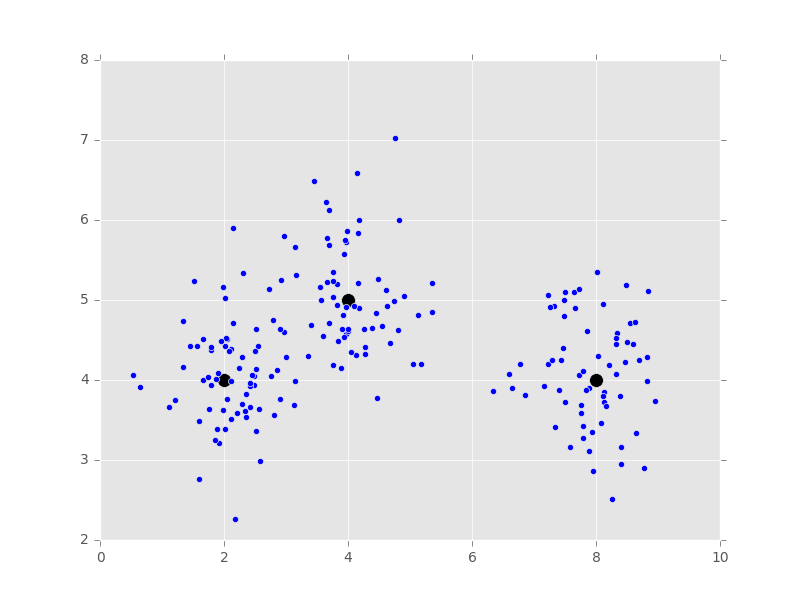
\includegraphics[scale = 0.5]{euclidean/figure_1.png}
		\end{figure}}
		
		\only<2>{\begin{figure}
				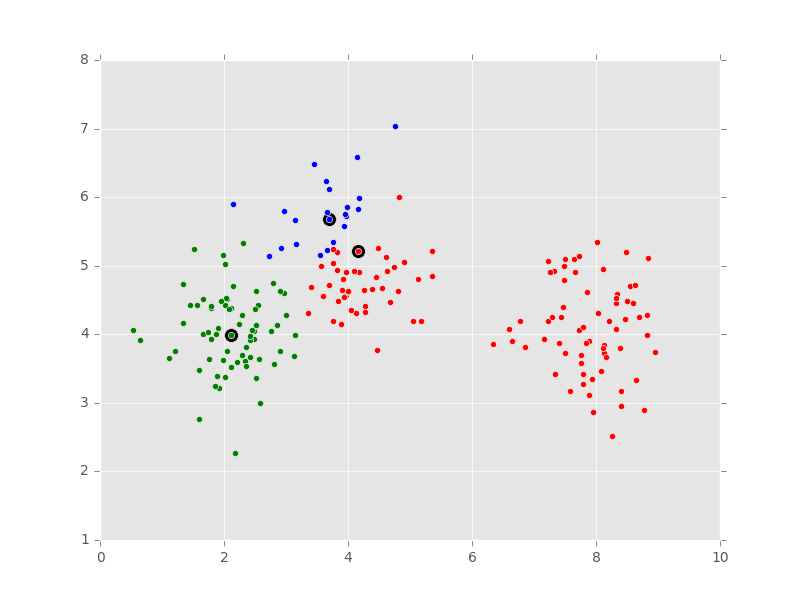
\includegraphics[scale = 0.5]{euclidean/figure_1-1.png}
			\end{figure}}	
			
		\only<3>{\begin{figure}
				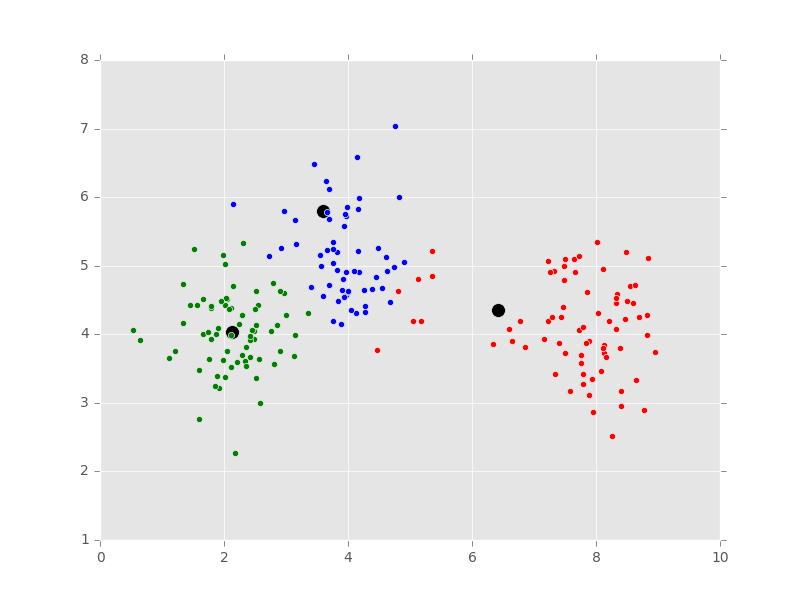
\includegraphics[scale = 0.5]{euclidean/figure_1-2.png}
			\end{figure}}
				
		\only<4>{\begin{figure}
					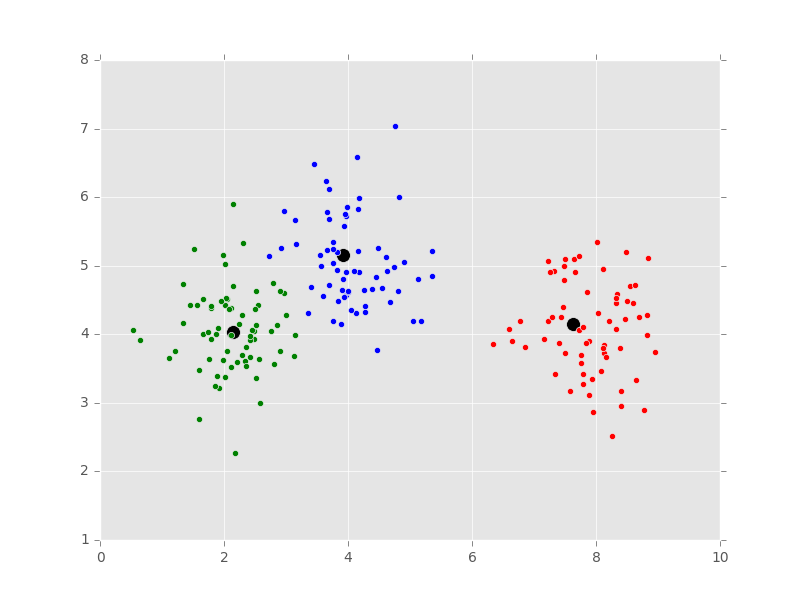
\includegraphics[scale = 0.5]{euclidean/figure_1-3.png}
				\end{figure}}	
		
		\only<5>{\begin{figure}
				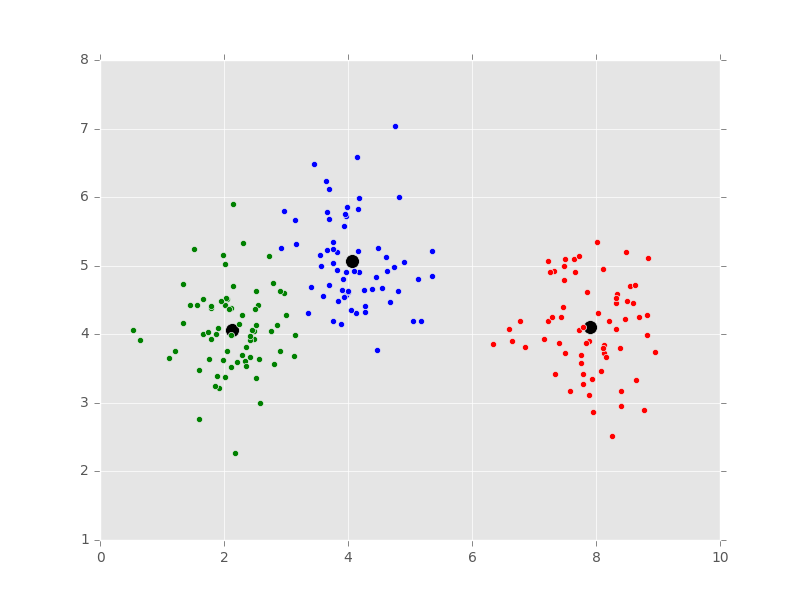
\includegraphics[scale = 0.5]{euclidean/figure_1-4.png}
			\end{figure}}			
			
		\only<6->{\begin{figure}
				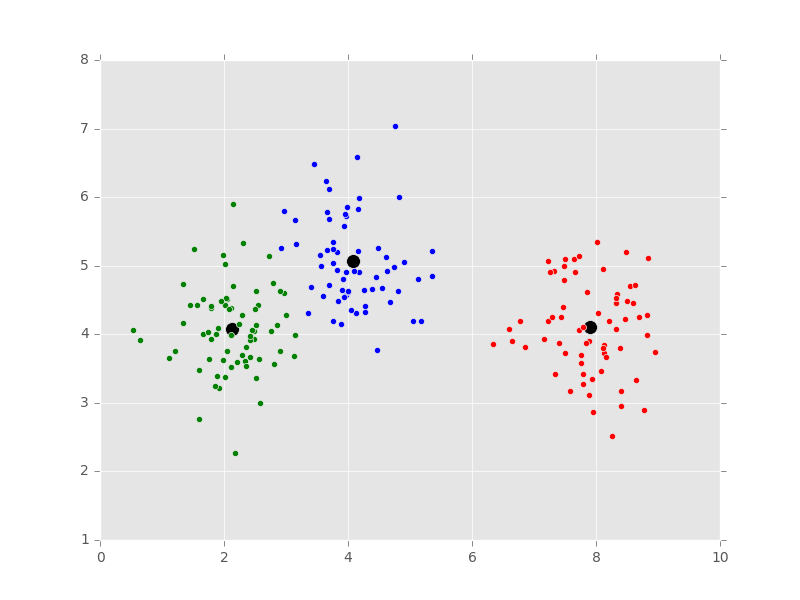
\includegraphics[scale = 0.5]{euclidean/figure_1-5.png}
			\end{figure}}	
				
\end{frame}


\section{Manhattan distance}
\begin{frame}{Manhattan distance}
$$ d(x,y) = \sum_{i}^{n} |x_i-y_i| $$	
\end{frame}


\begin{frame}{Manhattan distance}
	\only<1>{
		\begin{figure}
			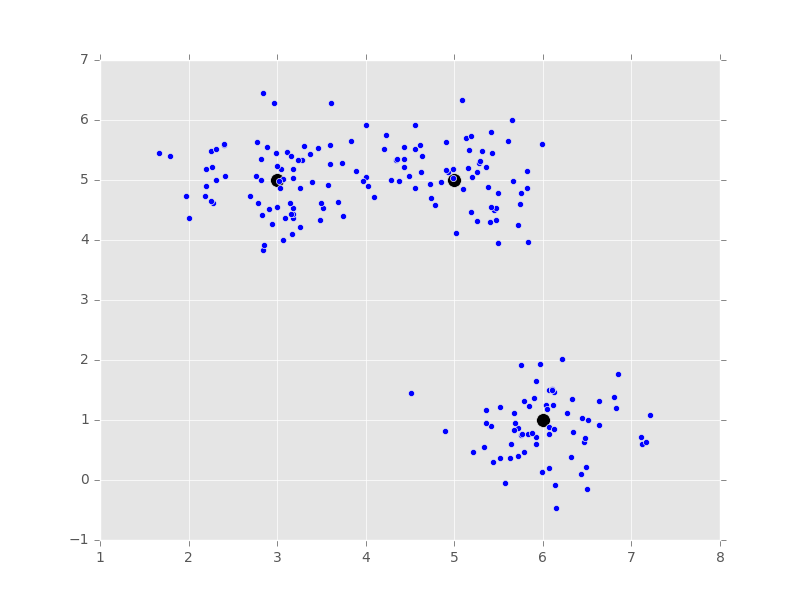
\includegraphics[scale = 0.5]{manhattan/figure_1.png}
		\end{figure}}
		
		\only<2>{\begin{figure}
				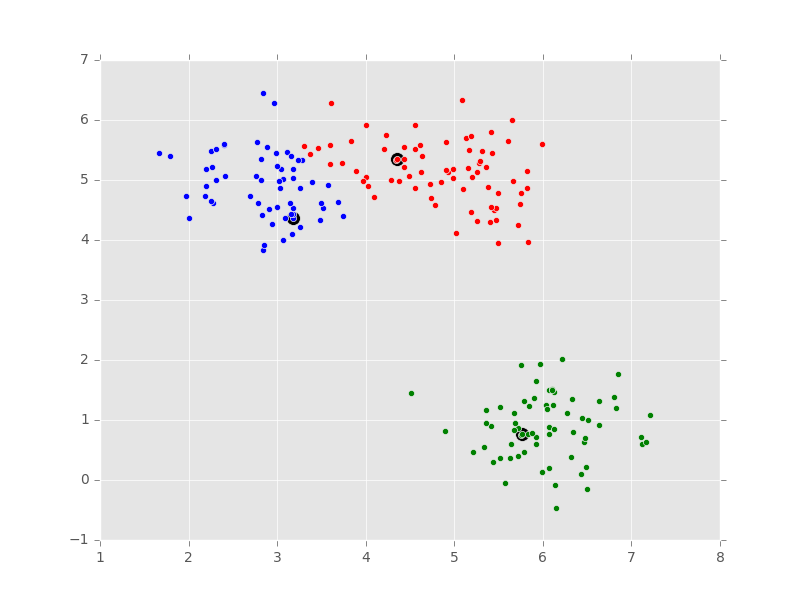
\includegraphics[scale = 0.5]{manhattan/figure_1-1.png}
			\end{figure}}	
			
			\only<3>{\begin{figure}
					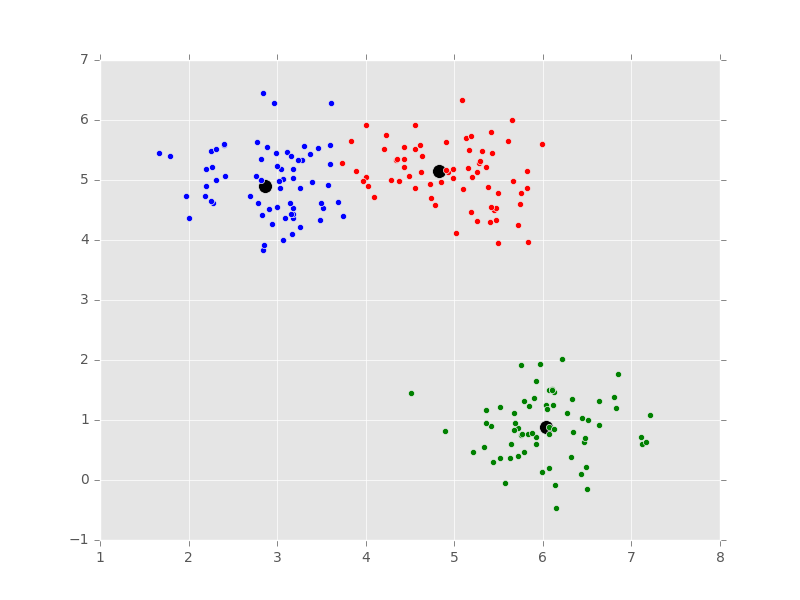
\includegraphics[scale = 0.5]{manhattan/figure_1-2.png}
				\end{figure}}
				
				\only<4>{\begin{figure}
						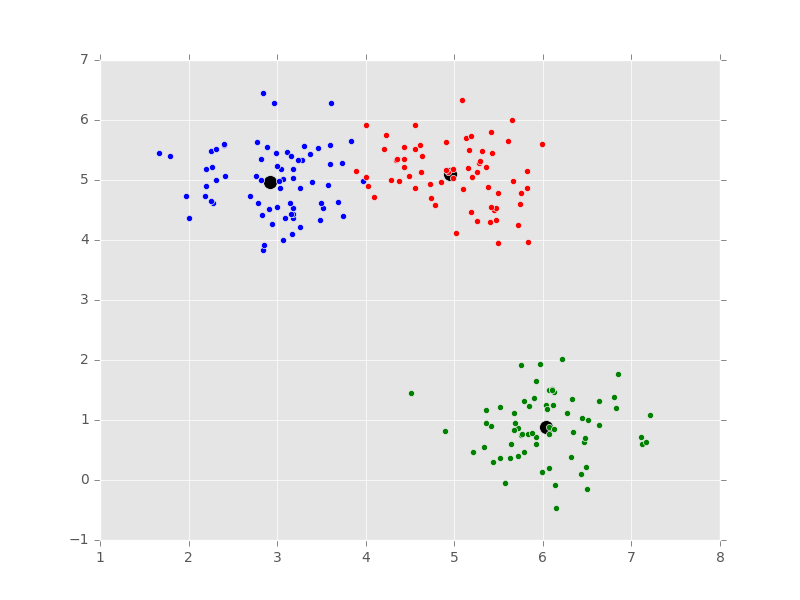
\includegraphics[scale = 0.5]{manhattan/figure_1-3.png}
					\end{figure}}	
					
					\only<5>{\begin{figure}
							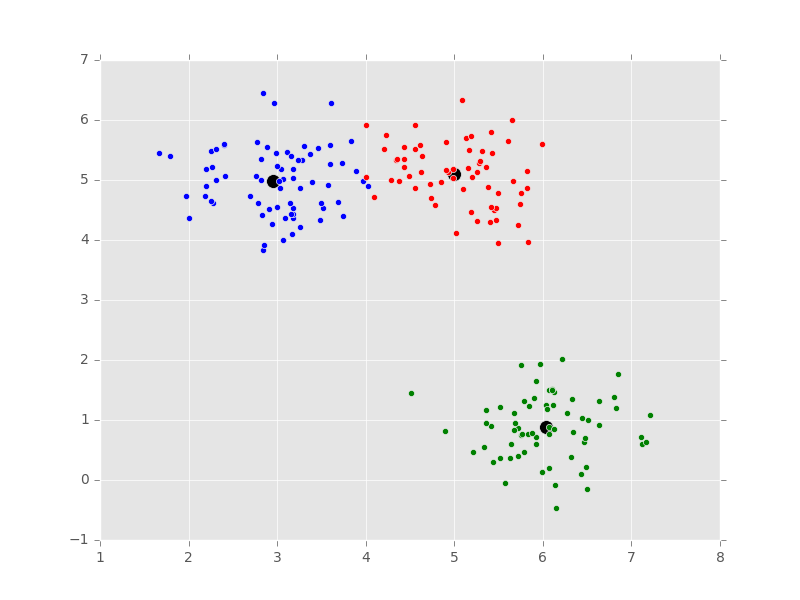
\includegraphics[scale = 0.5]{manhattan/figure_1-4.png}
						\end{figure}}			
						
						\only<6->{\begin{figure}
								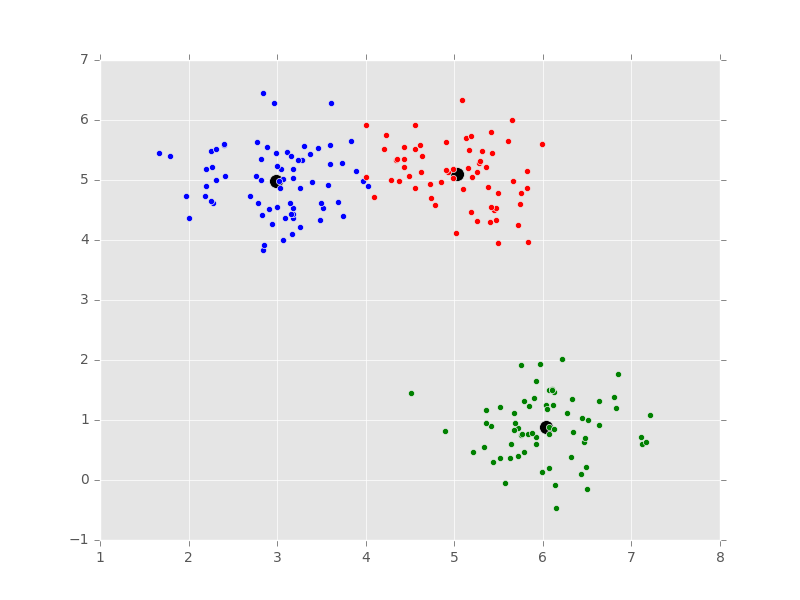
\includegraphics[scale = 0.5]{manhattan/figure_1-5.png}
							\end{figure}}	
\end{frame}						

\end{document}


\grid
\grid
